\chapter{System Design}

\subsection{How This Idea Was Designed}
I developed this application using my knowledge of Ionic and Firebase with past projects and labs conducted in the environment of GMIT. Not to mention also having the aid of online resources for different functionality and design to help with the project. The Ionic Framework helped with designing the project while past projects on GitHub and a mixture of online resources and video tutorials aided in the functionality of the application. The applications functionality was developed through a back end and front end using the unique Firebase Configuration.
\newline

The back end handling the Firebase Database stuff, in this case the authentication and crud functionality was handled here working in the background of the application. It stores the users on the Firebase website after a registration is made. Staff cannot access the applications main frame until they have verified their email, which may be in their junk/spam folder of there preferred email. It stores the data read in by the staff member, in this case the product details, note this form was implemented for prototype purposes.
\newline 

The front end is what the user of the application sees, so the design of the application, all the food groups, staff log in, staff log out, staff register and so on, here you can see the work of the back end, you can see the data read in from the Firebase Database showing the data read in by the user. The form in this application is for prototype reasons which i have mentioned above, in the application I envision potentially partnering with the retail till and shop stock database company CBE it will only show the products as the delivery dockets are read into CBE's system as already mentioned. 
\newpage
\subsection{Application Sketches and Diagrams}
These sketches below were drawn before the software development started in which were brought to meetings with the project supervisor. 
\newline
As you can see in the sketch below, this is a sketch of the home page when the application is ran. This is the first page the user is presented with.

\begin{figure}[h!]
	\caption{Design Sketch 1}
	\label{image:sketch1}
	\centering
	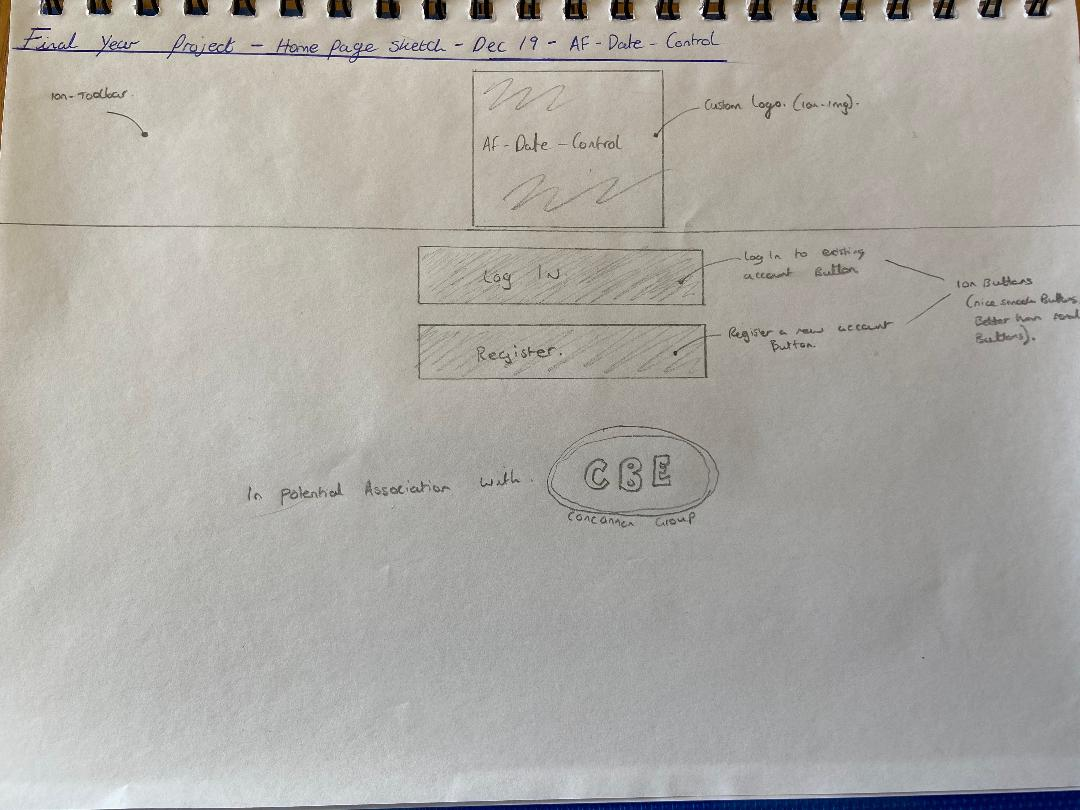
\includegraphics[width=0.7\textwidth]{images/sketch1.jpg}
\end{figure}

Here is a design sketch of the dashboard when the user signs in to their account:

\begin{figure}[h!]
	\caption{Design Sketch 2}
	\label{image:sketch2}
	\centering
	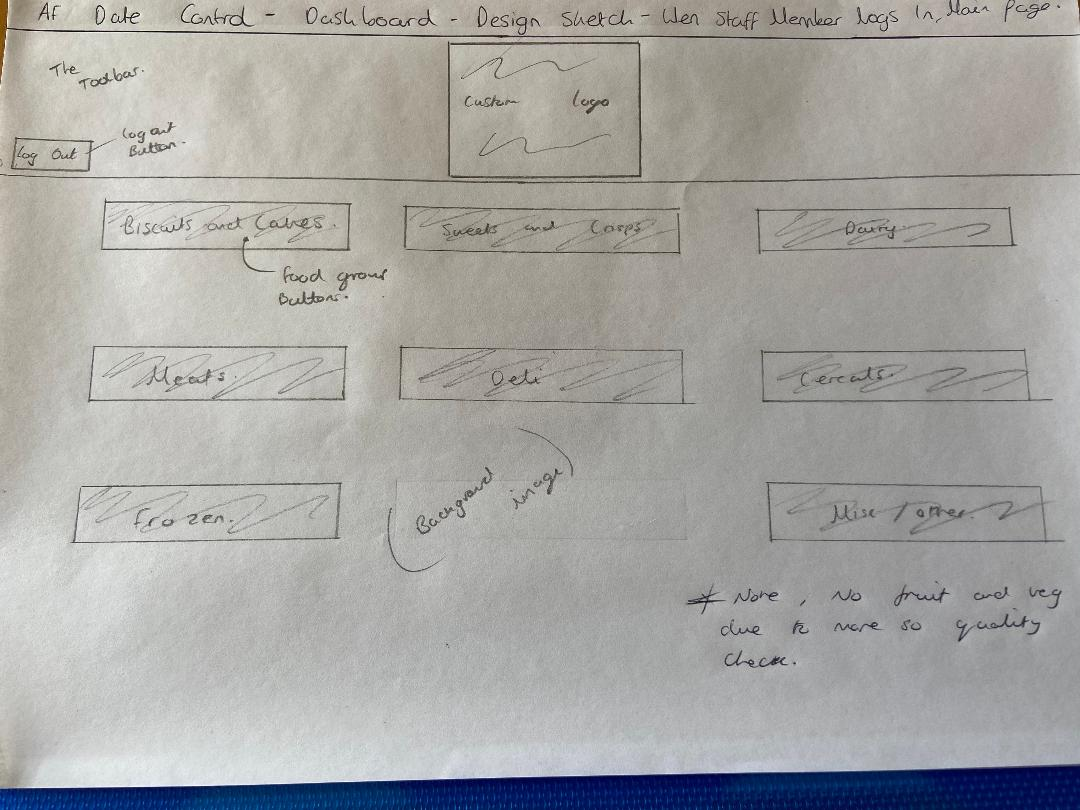
\includegraphics[width=0.7\textwidth]{images/sketch2.jpg}
\end{figure}
\newpage
Sketch of the product inventory page, add product form and product details.
\begin{figure}[h!]
	\caption{Design Sketch 3}
	\label{image:sketch3}
	\centering
	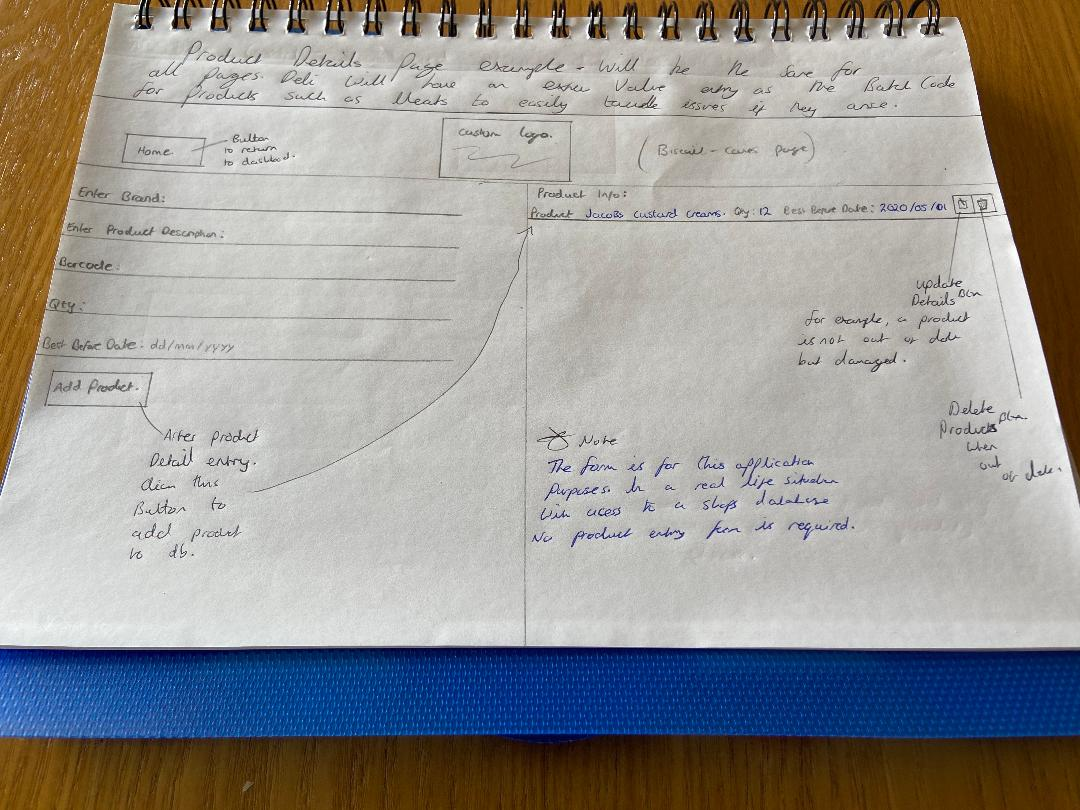
\includegraphics[width=0.5\textwidth]{images/sketch3.jpg}
\end{figure}

Below is a sketch of a functionality tree of the application
\begin{figure}[h!]
	\caption{Design Sketch 4}
	\label{image:sketch4}
	\centering
	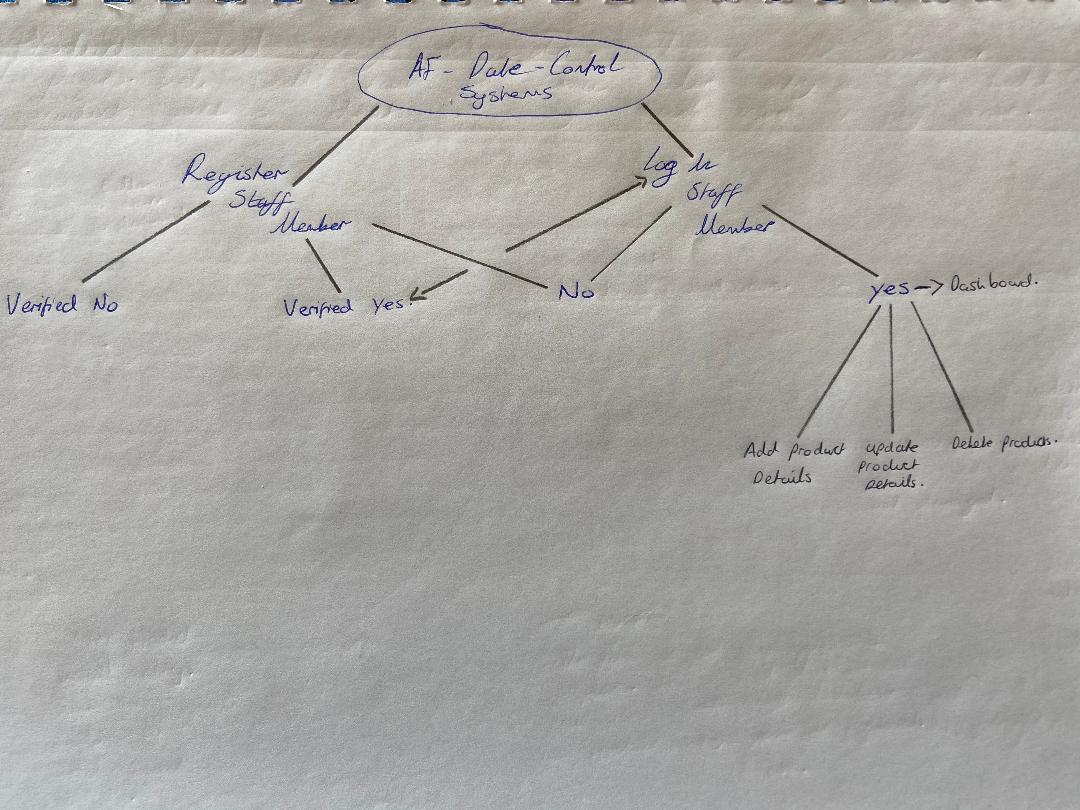
\includegraphics[width=0.5\textwidth]{images/sketch4.jpg}
\end{figure}

Finally a miniature UML diagram sketch of the application. 

\begin{figure}[h!]
	\caption{Design Sketch 5}
	\label{image:sketch5}
	\centering
	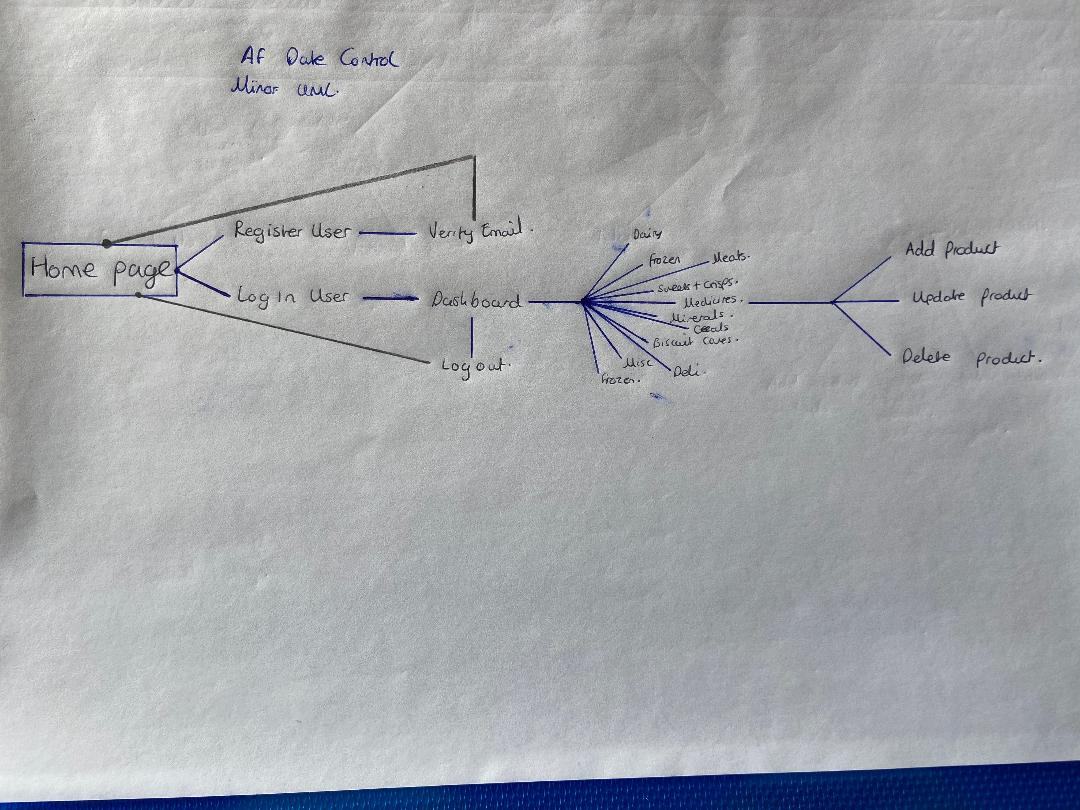
\includegraphics[width=0.5\textwidth]{images/sketch5.jpg}
\end{figure}
\newpage

\subsection{Application Design and Why}
For this Project Prototype Ionic Design Framework was used such as Ion Buttons, Ion Content and Ion Rows. Personally I love the look and smooth functionality of the output of Ionic Tags in HTML of the applications developed before. This was one of the main reasons for the switch to Ionic from Angular as mentioned in the above Technical Review of the project. 
\newline

The design of this project needed to be aesthetically pleasing for the user/staff member. It needed to show what the application revolved around, with a nice retail type background and color coded buttons for each high and low risk of passing its sell by date. I tried to implement images as buttons for the food groups as recommended by the project supervisor, however the end result wasn't what was envisioned from the outset. This application is for staff, not just anyone, they want quick viewing and easy to identify buttons for each divided food group. You will notice when testing this application that the fruit and vegetables section was left out, as mentioned above, fruit and vegetables vary, the majority do not have sell by dates, this is examined by the selling factor of the particular fruit. Would you buy it, if no it is wasted otherwise it stays where it is. I included a misc section for the fruit and vegetables products that have sell by dates but also for product groups not mentioned such as baby food and formulas and health and beauty products which you might find surprising to have a sell by date. The main aim of this application is to make it easy to understand and use for the staff member. Making it too complicated will result in the staff member maybe refusing to use it and go back to the habit of only physically checking by checking every item which is proven to be time consuming.
\newline

Features were added to this application for prototype purposes only as mentioned numerous times throughout this dissertation. The purpose is to show CBE that time and money could be saved in solving a problem within the workplace of retail in stock controlling. If they were to implement this idea, in which I have contacted an employee of CBE who was first conversed with at the careers fair in GMIT last winter to hopefully present this application and even let them test the application if they so wish. In the actual application if they were to implement this would possibly see changes to the application developed and remove prototype functions such as user authentication for staff, the form for entering in the product details and maybe change the food groups and types and even how they show the data stored in the cloud, which in their case would be the specific database for that particular shop. 
\newline 

\newpage
The promising aspect of this application, is it's flexibility, it can be used in various different ways, for example it can be used to keep track and compare with the HACCP sheets we have to fill in every time an item is taken off the shelf, or even be transformed in to an application that allows the user to record what is no longer on sale or in back stock to be ordered, the manager will then see this and order what is needed saving him/her time and the shop money in the process.

\begin{figure}[h!]
	\caption{Example of HACCP Sheet in the workplace}
	\label{image:HACCP}
	\centering
	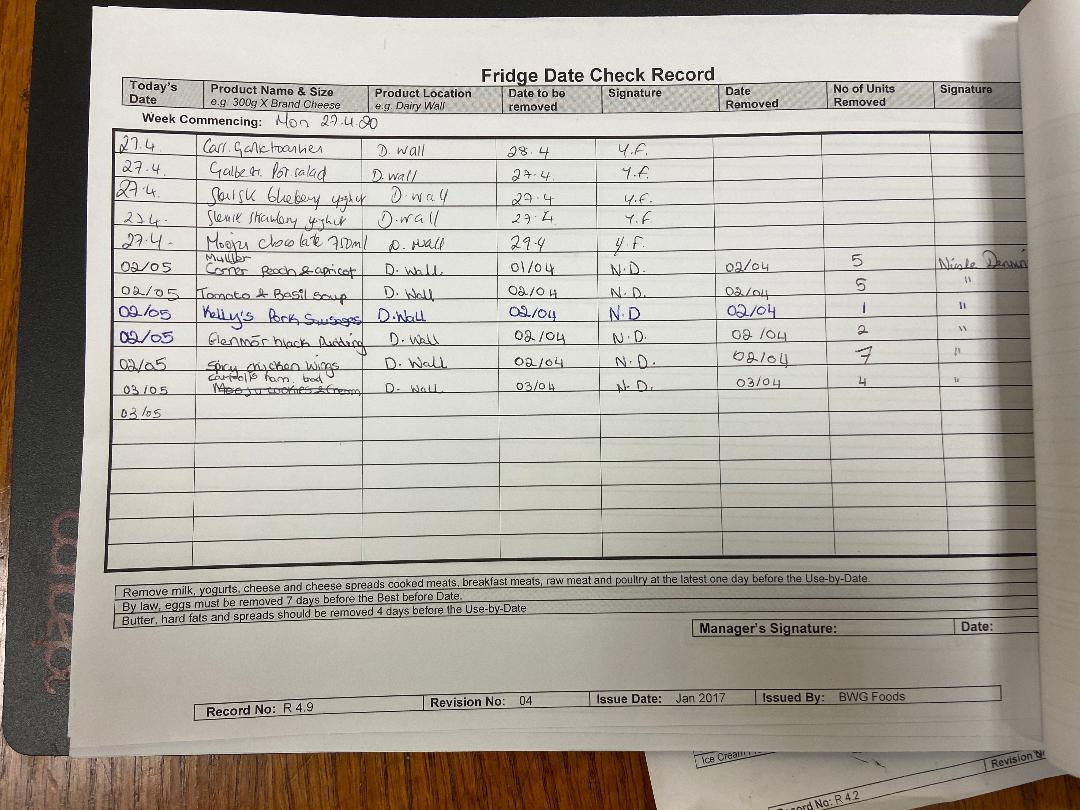
\includegraphics[width=0.9\textwidth]{images/HACCP.jpg}
\end{figure}

This application will help hugely in stock control and date checking sufficiency when it comes to HACCP sheets as it will give more a accurate indication of what is going off regularly to allow managers to improve tactical ordering of products. If a product continues to keep going out of date with not much sales this application and HACCP record will allow for the manager to not order as much or not order that product again.
\newline

This proves this applications flexibility and shows that it can help suppress more than one issue. It proves it can save time for the staff member and save the shop money in terms of tactical buying. Issues will always be present but its about reducing these issues in the workplace as much as possible, in which i believe this application will do so. 


\subsection{Self-Learned Extras}
In every project given or up taken throughout the four years of study in GMIT I learned something new in every project. Something new about each programming language, the different functions of cloud databases and local databases. All learnt throughout the four years has culminated into this project, this was the chance to show what I have learned and what was liked and disliked. Even using particular past projects to help with this final year project. I learned more about Firebase and Ionic while doing this project. For example In terms of user authentication with Ionic Firebase I learnt how to implement email verification into an application where once a user registers an account they are not permitted to sign in unless their email is verified. Learning also how to make the Ionic Firebase application a Firebase hosted website which saves so much time in terms of running the application and after making the application a website which turned about to be very satisfying. This is a huge factor going forward if I were to further develop this project or any new project for that matter as I enjoy this framework. 
